\documentclass{standalone}
\usepackage{tikz}
\usetikzlibrary{patterns, positioning}
\usepackage[sfdefault]{ClearSans} %% option 'sfdefault' activates Clear Sans as the default text font
\usepackage[T1]{fontenc}

\begin{document}
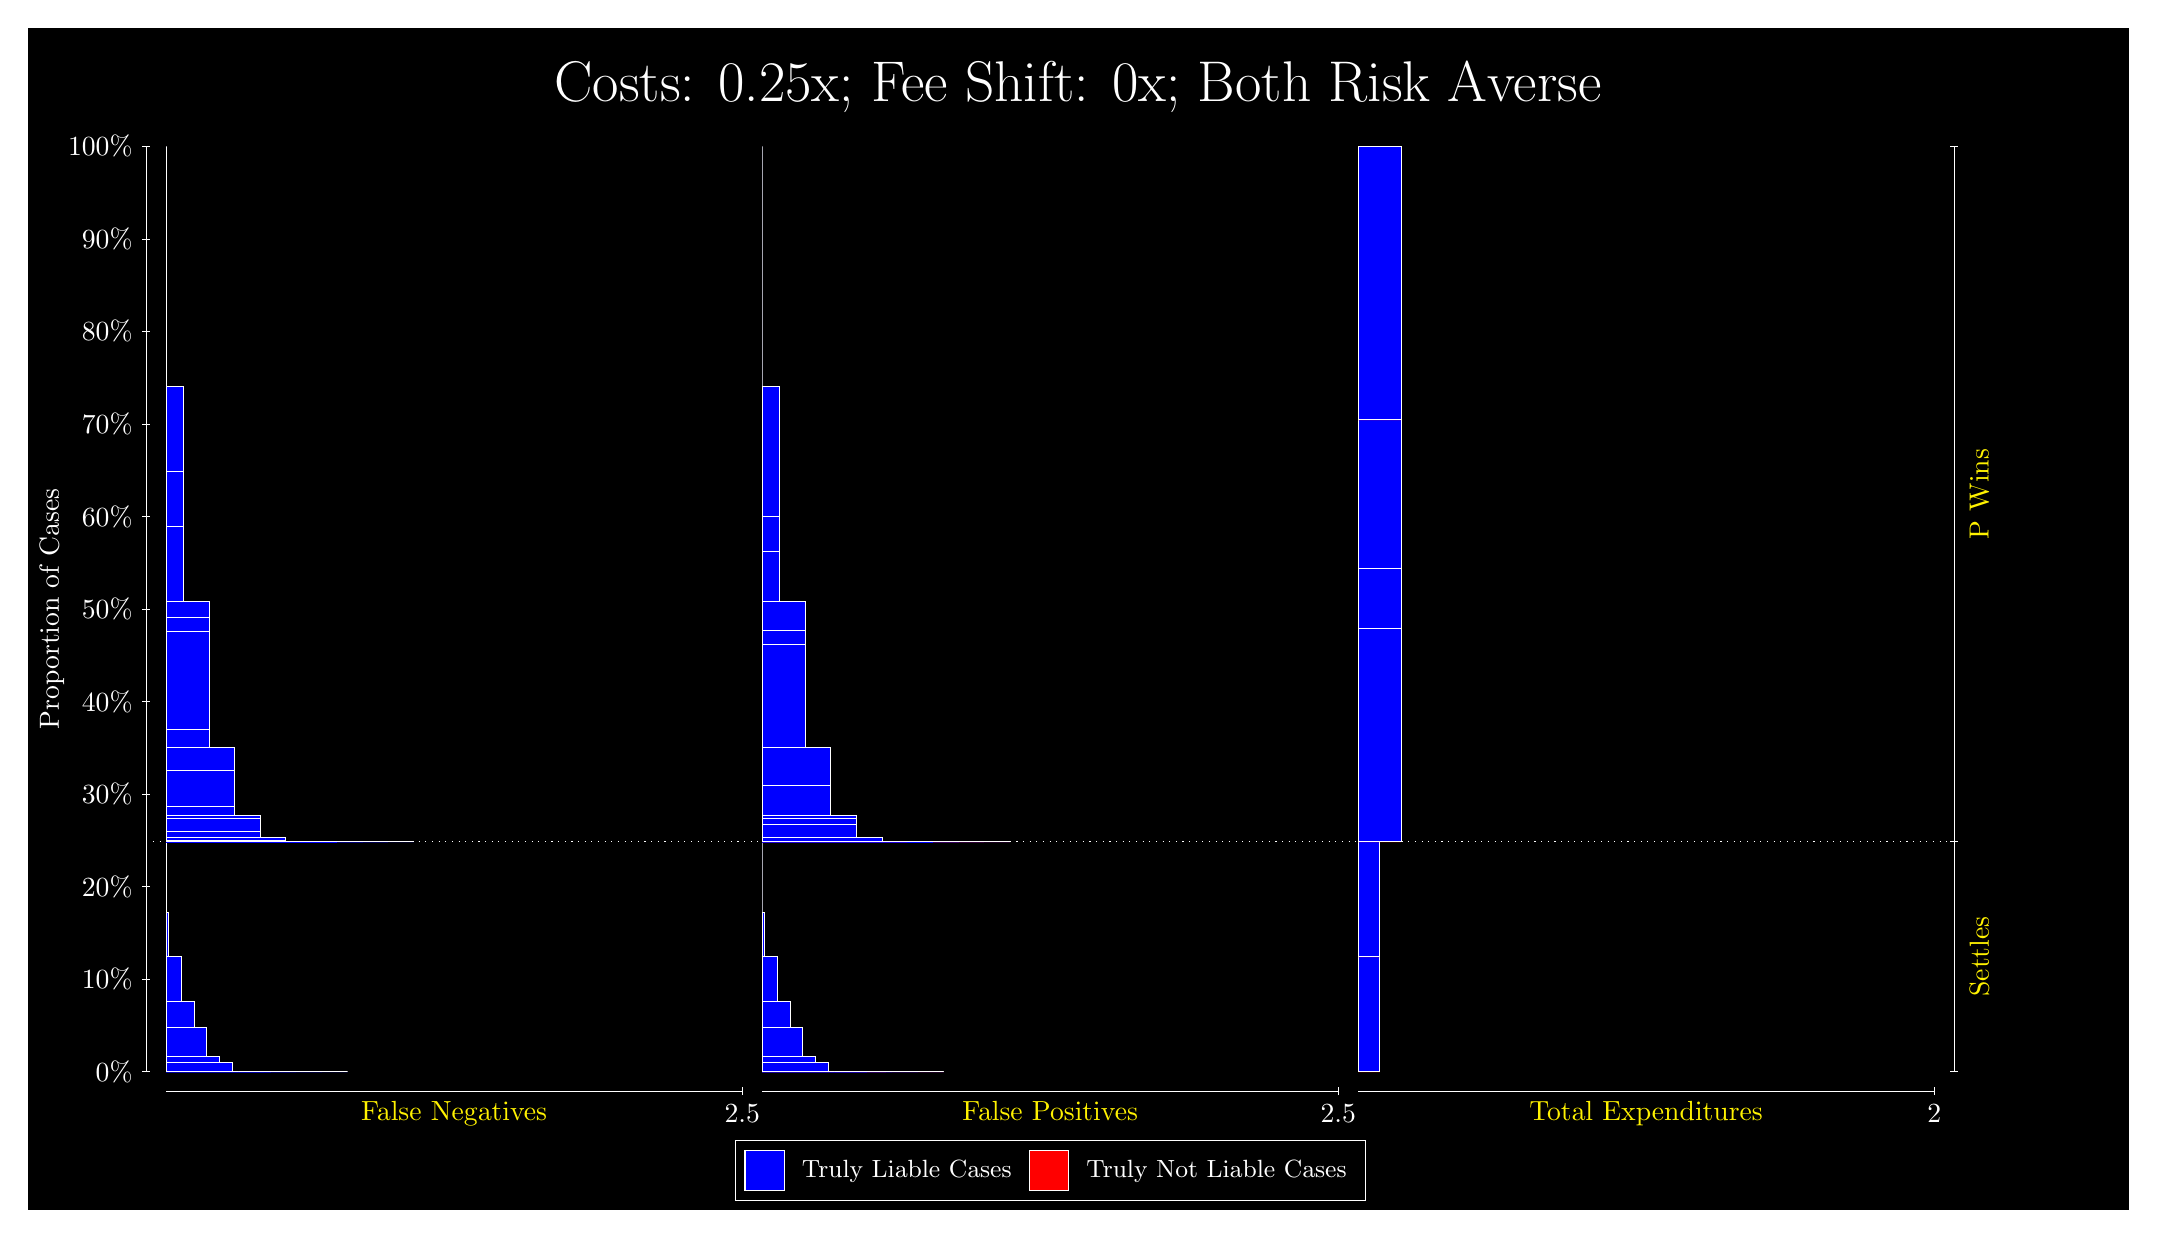
\begin{tikzpicture}
\draw[fill=black] (0,0) rectangle (26.667,15);
\draw[text=white] (0,13.5) rectangle (26.667,15) node[midway] {\huge Costs: 0.25x; Fee Shift: 0x; Both Risk Averse};
\draw[white, very thin] (1.5,1.75) -- (1.5,13.5);
\node[rotate=90, text=white, anchor=center] at (0.3, 7.625) {Proportion of Cases};
\draw[white, very thin] (1.45,1.75) -- (1.55,1.75);
\node[text=white, anchor=east] at (1.45, 1.75) {0\%};
\draw[white, very thin] (1.45,2.925) -- (1.55,2.925);
\node[text=white, anchor=east] at (1.45, 2.925) {10\%};
\draw[white, very thin] (1.45,4.1) -- (1.55,4.1);
\node[text=white, anchor=east] at (1.45, 4.1) {20\%};
\draw[white, very thin] (1.45,5.275) -- (1.55,5.275);
\node[text=white, anchor=east] at (1.45, 5.275) {30\%};
\draw[white, very thin] (1.45,6.45) -- (1.55,6.45);
\node[text=white, anchor=east] at (1.45, 6.45) {40\%};
\draw[white, very thin] (1.45,7.625) -- (1.55,7.625);
\node[text=white, anchor=east] at (1.45, 7.625) {50\%};
\draw[white, very thin] (1.45,8.8) -- (1.55,8.8);
\node[text=white, anchor=east] at (1.45, 8.8) {60\%};
\draw[white, very thin] (1.45,9.975) -- (1.55,9.975);
\node[text=white, anchor=east] at (1.45, 9.975) {70\%};
\draw[white, very thin] (1.45,11.15) -- (1.55,11.15);
\node[text=white, anchor=east] at (1.45, 11.15) {80\%};
\draw[white, very thin] (1.45,12.325) -- (1.55,12.325);
\node[text=white, anchor=east] at (1.45, 12.325) {90\%};
\draw[white, very thin] (1.45,13.5) -- (1.55,13.5);
\node[text=white, anchor=east] at (1.45, 13.5) {100\%};

\draw[white, very thin] (24.457,1.75) -- (24.457,13.5);
\draw[white, very thin] (24.407,1.75) -- (24.507,1.75);
\node[anchor=west] at (24.407, 1.75) {};
\draw[white, very thin] (24.407,4.6703) -- (24.507,4.6703);
\node[anchor=west] at (24.407, 4.6703) {};
\draw[white, very thin] (24.407,13.5) -- (24.507,13.5);
\node[anchor=west] at (24.407, 13.5) {};

\draw[white, very thin, fill=blue] (1.75,1.75) rectangle (4.0554,1.75);
\draw[white, very thin, fill=blue] (1.75,1.75) rectangle (3.7302,1.75);
\draw[white, very thin, fill=blue] (1.75,1.75) rectangle (3.4049,1.75);
\draw[white, very thin, fill=blue] (1.75,1.75) rectangle (3.3236,1.75);
\draw[white, very thin, fill=blue] (1.75,1.75) rectangle (3.0796,1.7502);
\draw[white, very thin, fill=blue] (1.75,1.7502) rectangle (2.9983,1.7502);
\draw[white, very thin, fill=blue] (1.75,1.7502) rectangle (2.7543,1.757);
\draw[white, very thin, fill=blue] (1.75,1.757) rectangle (2.673,1.757);
\draw[white, very thin, fill=blue] (1.75,1.757) rectangle (2.5917,1.8695);
\draw[white, very thin, fill=blue] (1.75,1.8695) rectangle (2.429,1.947);
\draw[white, very thin, fill=blue] (1.75,1.947) rectangle (2.3477,1.9471);
\draw[white, very thin, fill=blue] (1.75,1.9471) rectangle (2.2664,2.3078);
\draw[white, very thin, fill=blue] (1.75,2.3078) rectangle (2.1037,2.6459);
\draw[white, very thin, fill=blue] (1.75,2.6459) rectangle (2.0224,2.6464);
\draw[white, very thin, fill=blue] (1.75,2.6464) rectangle (1.9411,3.2102);
\draw[white, very thin, fill=blue] (1.75,3.2102) rectangle (1.7785,3.7739);
\draw[white, very thin, fill=red] (1.75,3.7739) rectangle (1.75,3.7739);
\draw[white, very thin, fill=blue] (1.75,3.7739) rectangle (1.75,4.6703);
\draw[white, very thin, fill=blue] (1.75,4.6703) rectangle (4.8971,4.6703);
\draw[white, very thin, fill=blue] (1.75,4.6703) rectangle (4.5718,4.6703);
\draw[white, very thin, fill=blue] (1.75,4.6703) rectangle (4.5718,4.6703);
\draw[white, very thin, fill=blue] (1.75,4.6703) rectangle (4.2465,4.6703);
\draw[white, very thin, fill=blue] (1.75,4.6703) rectangle (4.2465,4.6703);
\draw[white, very thin, fill=blue] (1.75,4.6703) rectangle (3.9213,4.6707);
\draw[white, very thin, fill=blue] (1.75,4.6707) rectangle (3.9213,4.6708);
\draw[white, very thin, fill=blue] (1.75,4.6708) rectangle (3.596,4.6772);
\draw[white, very thin, fill=blue] (1.75,4.6772) rectangle (3.2707,4.6919);
\draw[white, very thin, fill=blue] (1.75,4.6919) rectangle (3.2707,4.7307);
\draw[white, very thin, fill=blue] (1.75,4.7307) rectangle (2.9454,4.7966);
\draw[white, very thin, fill=blue] (1.75,4.7966) rectangle (2.9454,4.9662);
\draw[white, very thin, fill=blue] (1.75,4.9662) rectangle (2.9454,5.0029);
\draw[white, very thin, fill=blue] (1.75,5.0029) rectangle (2.6201,5.124);
\draw[white, very thin, fill=blue] (1.75,5.124) rectangle (2.6201,5.5747);
\draw[white, very thin, fill=blue] (1.75,5.5747) rectangle (2.6201,5.8688);
\draw[white, very thin, fill=blue] (1.75,5.8688) rectangle (2.2948,6.0989);
\draw[white, very thin, fill=blue] (1.75,6.0989) rectangle (2.2948,7.337);
\draw[white, very thin, fill=blue] (1.75,7.337) rectangle (2.2948,7.5151);
\draw[white, very thin, fill=blue] (1.75,7.5151) rectangle (2.2948,7.7191);
\draw[white, very thin, fill=blue] (1.75,7.7191) rectangle (1.9696,8.6775);
\draw[white, very thin, fill=blue] (1.75,8.6775) rectangle (1.9696,9.3702);
\draw[white, very thin, fill=blue] (1.75,9.3702) rectangle (1.9696,10.451);
\draw[white, very thin, fill=red] (1.75,10.451) rectangle (1.75,10.451);
\draw[white, very thin, fill=blue] (1.75,10.451) rectangle (1.75,13.5);
\draw[white, very thin, fill=red] (9.3189,1.75) rectangle (11.624,1.75);
\draw[white, very thin, fill=blue] (9.3189,1.75) rectangle (11.624,1.75);
\draw[white, very thin, fill=blue] (9.3189,1.75) rectangle (11.299,1.75);
\draw[white, very thin, fill=blue] (9.3189,1.75) rectangle (10.974,1.75);
\draw[white, very thin, fill=red] (9.3189,1.75) rectangle (10.892,1.75);
\draw[white, very thin, fill=blue] (9.3189,1.75) rectangle (10.892,1.75);
\draw[white, very thin, fill=blue] (9.3189,1.75) rectangle (10.648,1.7502);
\draw[white, very thin, fill=blue] (9.3189,1.7502) rectangle (10.567,1.7502);
\draw[white, very thin, fill=blue] (9.3189,1.7502) rectangle (10.323,1.757);
\draw[white, very thin, fill=blue] (9.3189,1.757) rectangle (10.242,1.757);
\draw[white, very thin, fill=red] (9.3189,1.757) rectangle (10.161,1.757);
\draw[white, very thin, fill=blue] (9.3189,1.757) rectangle (10.161,1.8695);
\draw[white, very thin, fill=blue] (9.3189,1.8695) rectangle (9.9979,1.947);
\draw[white, very thin, fill=blue] (9.3189,1.947) rectangle (9.9166,1.9471);
\draw[white, very thin, fill=blue] (9.3189,1.9471) rectangle (9.8353,2.3078);
\draw[white, very thin, fill=blue] (9.3189,2.3078) rectangle (9.6726,2.6459);
\draw[white, very thin, fill=blue] (9.3189,2.6459) rectangle (9.5913,2.6464);
\draw[white, very thin, fill=blue] (9.3189,2.6464) rectangle (9.51,3.2101);
\draw[white, very thin, fill=blue] (9.3189,3.2101) rectangle (9.3473,3.7738);
\draw[white, very thin, fill=blue] (9.3189,3.7738) rectangle (9.3189,4.6703);
\draw[white, very thin, fill=red] (9.3189,4.6703) rectangle (12.466,4.6703);
\draw[white, very thin, fill=blue] (9.3189,4.6703) rectangle (12.466,4.6703);
\draw[white, very thin, fill=red] (9.3189,4.6703) rectangle (12.141,4.6703);
\draw[white, very thin, fill=blue] (9.3189,4.6703) rectangle (12.141,4.6703);
\draw[white, very thin, fill=red] (9.3189,4.6703) rectangle (11.815,4.6703);
\draw[white, very thin, fill=blue] (9.3189,4.6703) rectangle (11.815,4.6703);
\draw[white, very thin, fill=blue] (9.3189,4.6703) rectangle (11.815,4.6703);
\draw[white, very thin, fill=blue] (9.3189,4.6703) rectangle (11.49,4.6705);
\draw[white, very thin, fill=red] (9.3189,4.6705) rectangle (11.49,4.6705);
\draw[white, very thin, fill=blue] (9.3189,4.6705) rectangle (11.49,4.6708);
\draw[white, very thin, fill=red] (9.3189,4.6708) rectangle (11.165,4.6708);
\draw[white, very thin, fill=blue] (9.3189,4.6708) rectangle (11.165,4.6772);
\draw[white, very thin, fill=red] (9.3189,4.6772) rectangle (10.84,4.6772);
\draw[white, very thin, fill=blue] (9.3189,4.6772) rectangle (10.84,4.7307);
\draw[white, very thin, fill=red] (9.3189,4.7307) rectangle (10.514,4.7307);
\draw[white, very thin, fill=blue] (9.3189,4.7307) rectangle (10.514,4.8926);
\draw[white, very thin, fill=blue] (9.3189,4.8926) rectangle (10.514,4.9615);
\draw[white, very thin, fill=blue] (9.3189,4.9615) rectangle (10.514,5.0029);
\draw[white, very thin, fill=red] (9.3189,5.0029) rectangle (10.189,5.0029);
\draw[white, very thin, fill=blue] (9.3189,5.0029) rectangle (10.189,5.3907);
\draw[white, very thin, fill=blue] (9.3189,5.3907) rectangle (10.189,5.8688);
\draw[white, very thin, fill=red] (9.3189,5.8688) rectangle (9.8637,5.8688);
\draw[white, very thin, fill=blue] (9.3189,5.8688) rectangle (9.8637,7.1755);
\draw[white, very thin, fill=blue] (9.3189,7.1755) rectangle (9.8637,7.3536);
\draw[white, very thin, fill=blue] (9.3189,7.3536) rectangle (9.8637,7.7191);
\draw[white, very thin, fill=blue] (9.3189,7.7191) rectangle (9.5384,8.3601);
\draw[white, very thin, fill=red] (9.3189,8.3601) rectangle (9.5384,8.3601);
\draw[white, very thin, fill=blue] (9.3189,8.3601) rectangle (9.5384,8.8);
\draw[white, very thin, fill=blue] (9.3189,8.8) rectangle (9.5384,10.451);
\draw[white, very thin, fill=blue] (9.3189,10.451) rectangle (9.3189,13.5);
\draw[white, very thin, fill=red] (16.888,1.75) rectangle (17.162,1.75);
\draw[white, very thin, fill=blue] (16.888,1.75) rectangle (17.162,3.2095);
\draw[white, very thin, fill=red] (16.888,3.2095) rectangle (17.162,3.2095);
\draw[white, very thin, fill=blue] (16.888,3.2095) rectangle (17.162,4.6703);
\draw[white, very thin, fill=red] (16.888,4.6703) rectangle (17.437,4.6703);
\draw[white, very thin, fill=blue] (16.888,4.6703) rectangle (17.437,7.3834);
\draw[white, very thin, fill=red] (16.888,7.3834) rectangle (17.437,7.3834);
\draw[white, very thin, fill=blue] (16.888,7.3834) rectangle (17.437,8.1413);
\draw[white, very thin, fill=red] (16.888,8.1413) rectangle (17.437,8.1413);
\draw[white, very thin, fill=blue] (16.888,8.1413) rectangle (17.437,10.029);
\draw[white, very thin, fill=red] (16.888,10.029) rectangle (17.437,10.029);
\draw[white, very thin, fill=blue] (16.888,10.029) rectangle (17.437,13.5);
\draw[white, dotted] (1.5,4.6703) -- (24.457,4.6703);
\draw[white, very thin] (1.75,1.5) -- (9.0689,1.5);
\node[text=yellow, anchor=north] at (5.4094, 1.5) {False Negatives};
\draw[white, very thin] (9.0689,1.45) -- (9.0689,1.55);
\node[text=white, anchor=north] at (9.0689, 1.45) {2.5};

\draw[white, very thin] (9.3189,1.5) -- (16.638,1.5);
\node[text=yellow, anchor=north] at (12.978, 1.5) {False Positives};
\draw[white, very thin] (16.638,1.45) -- (16.638,1.55);
\node[text=white, anchor=north] at (16.638, 1.45) {2.5};

\draw[white, very thin] (16.888,1.5) -- (24.207,1.5);
\node[text=yellow, anchor=north] at (20.547, 1.5) {Total Expenditures};
\draw[white, very thin] (24.207,1.45) -- (24.207,1.55);
\node[text=white, anchor=north] at (24.207, 1.45) {2};

\node[text=yellow, centered, rotate=90] at (24.777, 3.2101) {Settles};
\node[text=yellow, centered, rotate=90] at (24.777, 9.0851) {P Wins};

\draw (12.978300999999998,1.5) node[draw=none] (baseCoordinate) {};
\begin{scope}[align=center]
        \matrix[scale=0.5, draw=white, below=0.5cm of baseCoordinate, nodes={draw}, column sep=0.1cm]{
            \node[rectangle, draw, minimum width=0.5cm, minimum height=0.5cm, fill=blue] {}; &
            \node[draw=none, font=\small, text=white] (B) {Truly Liable Cases}; &
            \node[rectangle, draw, minimum width=0.5cm, minimum height=0.5cm, fill=red] {}; &
            \node[draw=none, font=\small, text=white] (B) {Truly Not Liable Cases}; \\
            };
\end{scope}

\end{tikzpicture}
\end{document}